\documentclass[12pt]{article}
%\usepackage[utf8]{inputenc}
\usepackage{indentfirst}
\usepackage{float}
\usepackage{array}
\usepackage{url}
\urlstyle{tt}
\usepackage{enumitem, amsmath, amssymb, amsfonts, latexsym, mathrsfs}
\usepackage{graphicx}
\usepackage{subfig}
\usepackage{multicol}
\usepackage{booktabs}
\usepackage{ragged2e}
\usepackage{svg}
\usepackage{xcolor}
\usepackage{tabularray}

\usepackage{listings}
\usepackage{atkinson} %% Option 'sfdefault' if the base
%% font of the document is to be sans serif.
\usepackage[T1]{fontenc}
\setmainfont{Atkinson Hyperlegible}
\renewcommand{\familydefault}{\sfdefault}

\usepackage[spanish]{babel}
\usepackage[utf8]{inputenc}
\usepackage[backend=biber]{biblatex}
\bibliography{referencias}
\usepackage{csquotes}
%New colors defined below
\usepackage{}
\definecolor{codegreen}{rgb}{0,0.6,0}
\definecolor{codegray}{rgb}{0.5,0.5,0.5}
\definecolor{codepurple}{rgb}{0.58,0,0.82}
\definecolor{backcolour}{rgb}{0.95,0.95,0.92}
\lstdefinestyle{mystyle}{
  backgroundcolor=\color{backcolour},   commentstyle=\color{codegreen},
  keywordstyle=\color{magenta},
  numberstyle=\tiny\color{codegray},
  stringstyle=\color{codepurple},
  basicstyle=\ttfamily\footnotesize,
  breakatwhitespace=false,         
  breaklines=true,                 
  captionpos=b,                    
  keepspaces=true,                 
  numbers=left,                    
  numbersep=5pt,                  
  showspaces=false,                
  showstringspaces=false,
  showtabs=false,                  
  tabsize=2
}
%"mystyle" code listing set
\lstset{style=mystyle}
%\lstset{basicstyle=\ttfamily\footnotesize,breaklines=true}

\usepackage{notoccite}

\usepackage{multicol}
\setlength{\columnseprule}{1pt}
\def\columnseprulecolor{\color{black}}





\date{}
% Comand para keywords
\providecommand{\keywords}[1]
{
  \small	
  \textbf{\textit{Keywords---}} #1
}

% Tipografía
%\usepackage{helvet}
%\renewcommand{\familydefault}{\sfdefault}
%\usepackage[sfdefault]{Chivo}
%\usepackage{comment}


\urlstyle{same}
% \tolerance=9999
% \emergencystretch=10pt
\hyphenpenalty=10000
\sloppy
% \exhyphenpenalty=100

\renewcommand{\figurename}{\textbf{Figura.}}
\renewcommand\spanishtablename{Tabla.}

% Interlineado
\usepackage{setspace}
\spacing{1.15}

% Márgenes
\usepackage[a4paper]{geometry}
\geometry{top=2.5cm, bottom=2.5cm, left=2cm, right=2cm}

% Número de página
\usepackage{fancyhdr}
\pagestyle{fancy}
\rhead[]{}
\lhead[]{}
\renewcommand{\headrulewidth}{0pt}
\rfoot[]{\thepage}
\cfoot[]{}

\usepackage[breaklinks]{hyperref}
% Setup de hiperenlaces
\hypersetup{
    colorlinks=true,
    linkcolor=blue,
    filecolor=magenta,      
    urlcolor=cyan,
    pdftitle={Arquitectura de las consolas de videojuegos},
    pdfpagemode=FullScreen,
    citecolor = green
    }
\usepackage[norule]{footmisc}

%_____________________________________________________________________________
%_____________________________________________________________________________
%_____________________________________________________________________________
%_____________________________________________________________________________
\hbadness=50000
\usepackage{microtype}
\begin{document}
\nocite{atkinson}
\nocite{circuitverse}
\nocite{chatgpt}
\nocite{duke}
% PORTADA        
\begin{titlepage}
        \begin{center}
             
         
        \hrule
        \vspace{1cm}
        %{\bfseries\Large UNIVERSIDAT JAUME I \par}
        \vspace{1cm}
        {\bfseries\huge Apuntes de Consolas y Dispositivos de Videojuegos \par}
        \vspace{2cm}

        \begin{figure}[H]
            \centering
            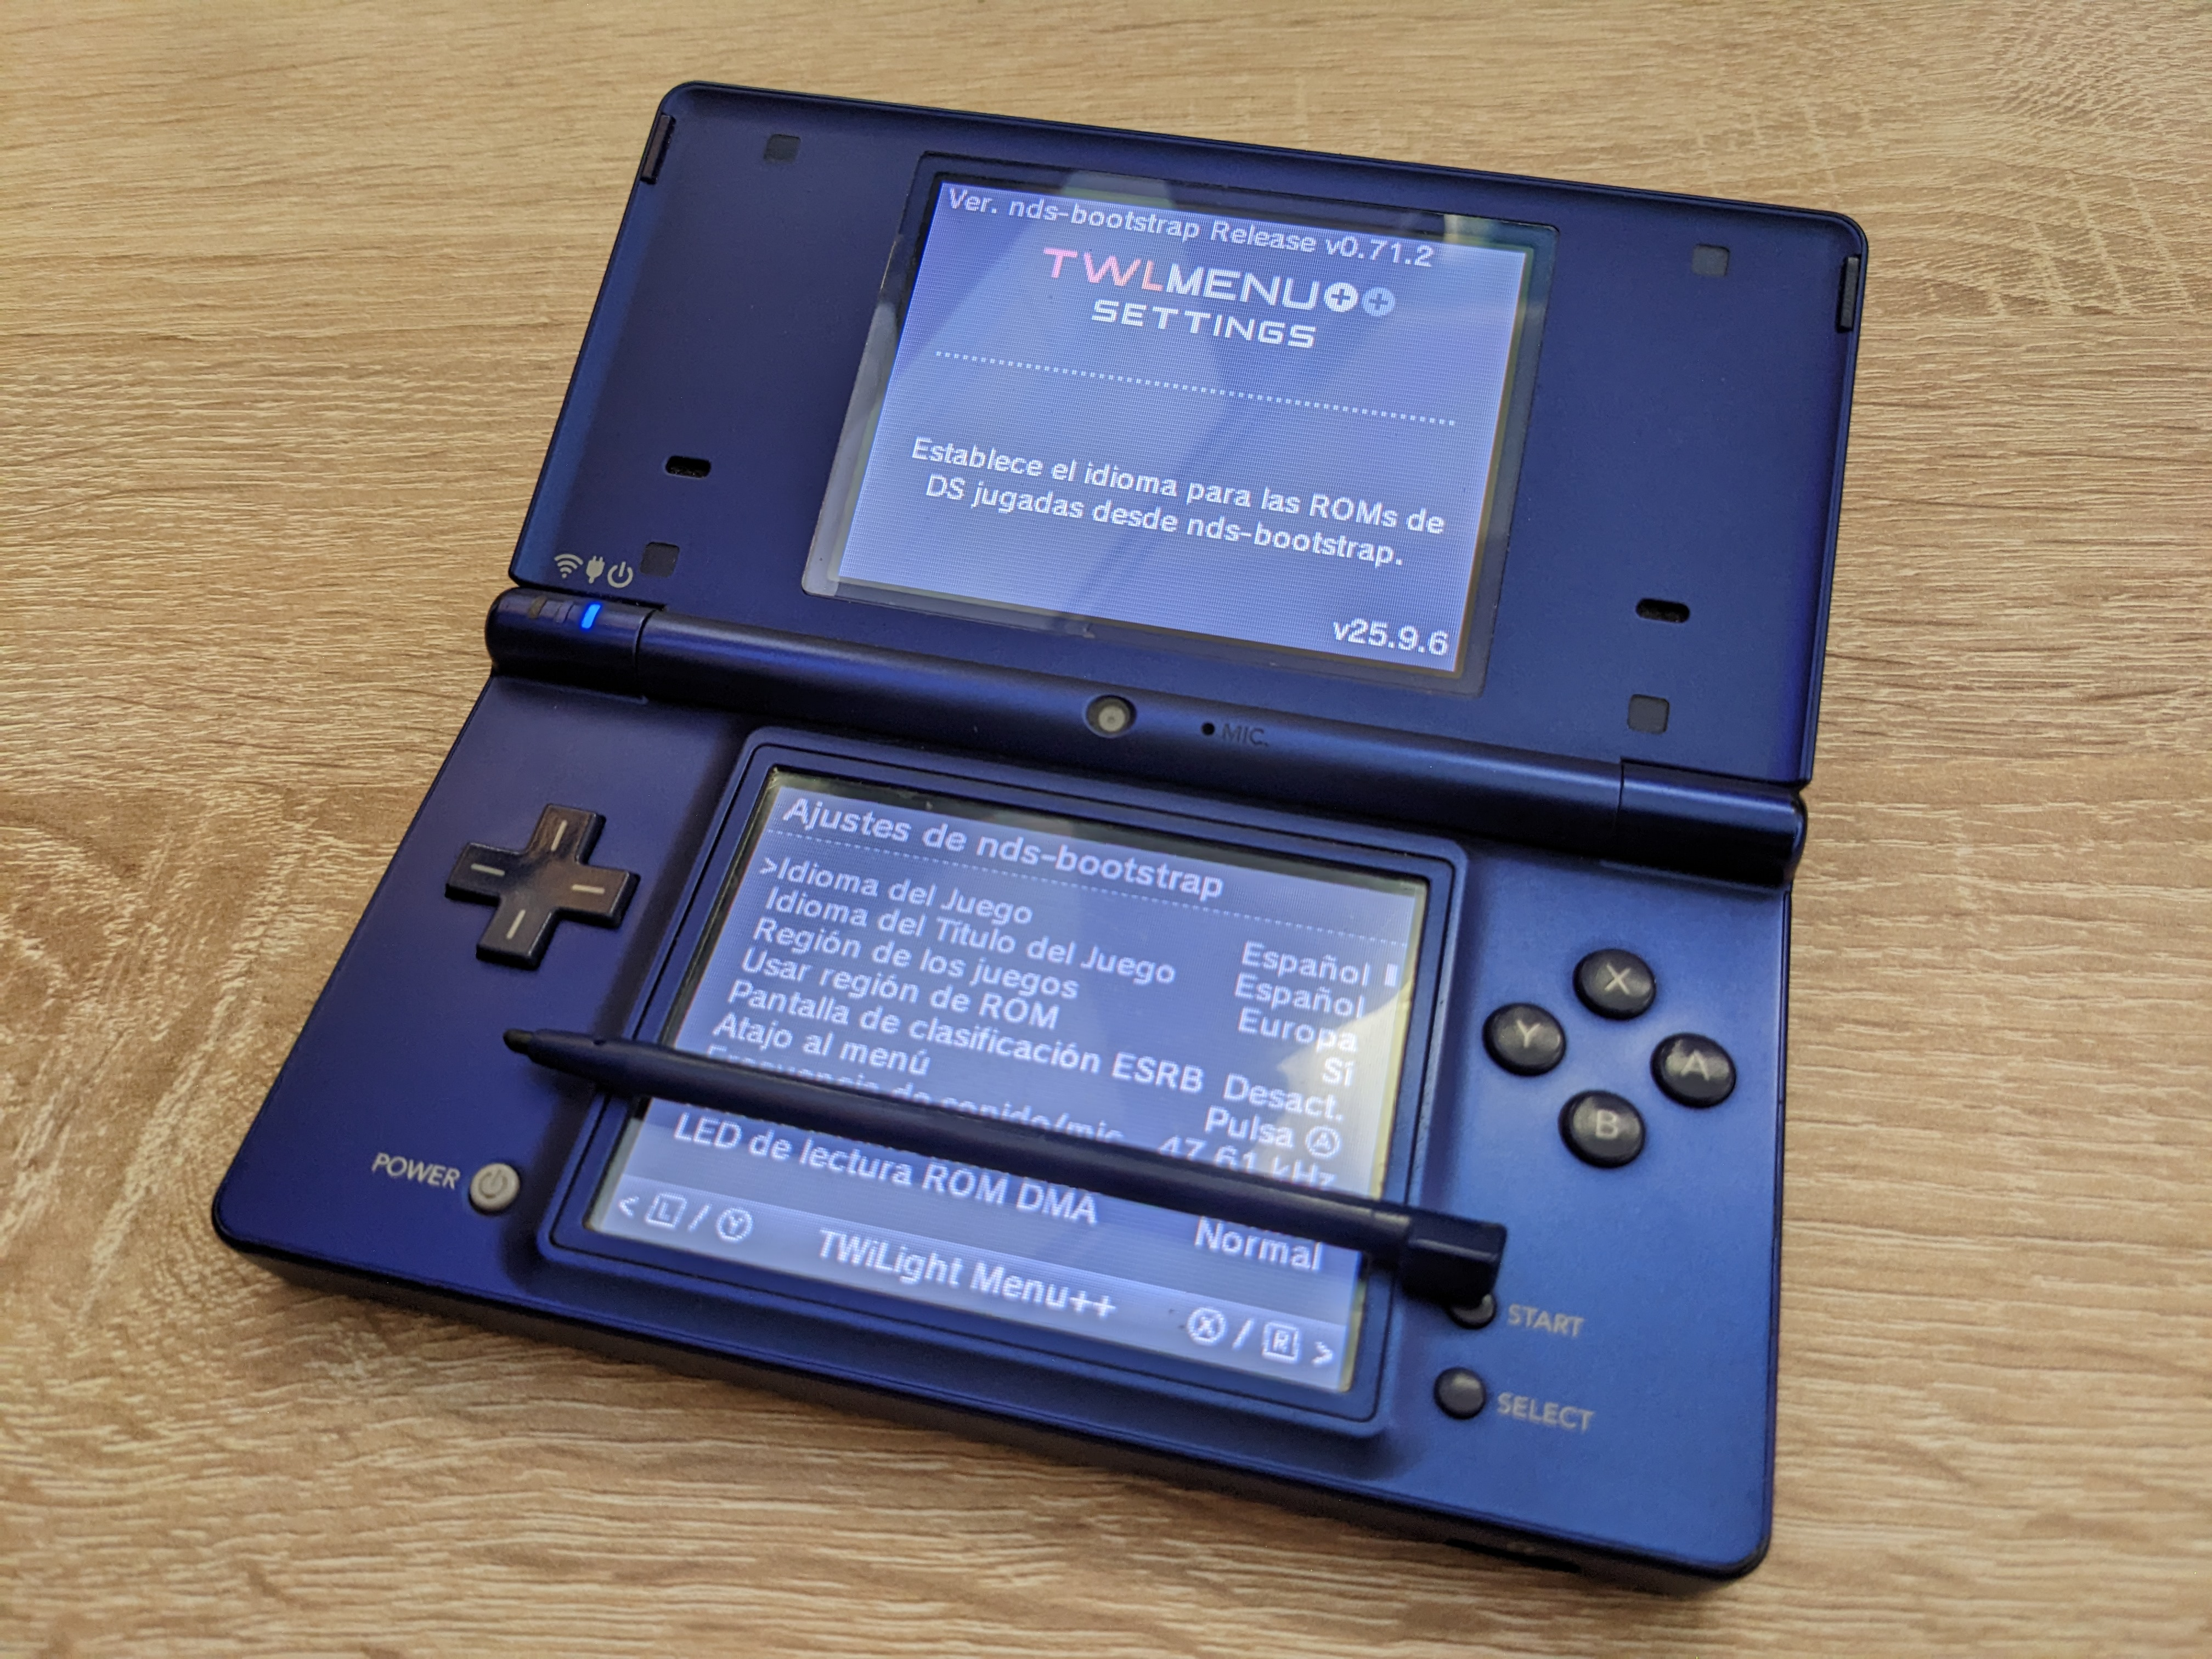
\includegraphics[width=\textwidth]{dsi.jpg}
            \caption*{\footnotesize{\textit{Nintendo DSi con Homebrew y emulador de NDS}}}
            \label{fig:dsi}
        \end{figure}
        
        {\large 
        Jesús Jiménez Montero \\
        \par}
        \vspace{1cm}
        \hrule
        \vspace{1cm}

        {\large 
        \textit{Versión 4: ALU\\
        Fecha: 09/10/2023}
        \par}
        \end{center}
\end{titlepage}

% ÍNDICE
%\renewcommand{\tableofcontents}{Indice general}
\newpage
\renewcommand{\contentsname}{Tabla de contenidos}
\setcounter{secnumdepth}{5}
\tableofcontents
\setcounter{tocdepth}{4}

\newpage
%-----------------------------------------------------------------
%-----------------------------------------------------------------
% Tabla de figuras
\newpage
\renewcommand{\listfigurename}{Lista de figuras}
\thispagestyle{empty}
\listoffigures
\newpage

\renewcommand{\listtablename}{Lista de tablas}
\listoftables
\newpage

%-----------------------------------------------------------------
%-----------------------------------------------------------------

%%%%%%%%%%%%%%%%%%%%%%%%%%%%%%%%%%%%%%%%%%%%%%%%%%%%%%%%%%%%%%%%%%%%%%%%%%
%%%%%%%%%%%%%%%%%%%%%%%%%%%%%%%%%%%%%%%%%%%%%%%%%%%%%%%%%%%%%%%%%%%%%%%%%%
\section{HalfAdder}
\hrule
\vspace{0.5cm}
    \subsection{Tabla de verdad y explicación del circuito}
        El Half-Adder hace la operación de adición de dos números binarios (dos bits) y da dos outputs, la suma de estos y el acarreo. 
        La suma se produce con dos puertas, un XOR, que lleva la suma y produce un 1 cuando A o B es 1, pero no ambos. Y una AND que produce 1 solamente cuando A y B son 1. 
        \begin{table}[H]
        \centering
        \caption{Tabla de verdad de HalfAdder}
        \label{tab:halfadder}
        \begin{tblr}{
          width = \linewidth,
          colspec = {Q[87]Q[87]Q[315]Q[350]},
          hline{1,6} = {-}{0.08em},
          hline{2} = {-}{0.05em},
        }
        \texttt{A} & \texttt{B} & \texttt{Sum (S)} & \texttt{Carry (C)} \\
        \texttt{0} & \texttt{0} & \texttt{0}       & \texttt{0}         \\
        \texttt{0} & \texttt{1} & \texttt{1}       & \texttt{0}         \\
        \texttt{1} & \texttt{0} & \texttt{1}       & \texttt{0}         \\
        \texttt{1} & \texttt{1} & \texttt{0}       & \texttt{1}         
        \end{tblr}
        \end{table}

    \subsection{Esquema del circuito exterior y exterior} 
        \begin{figure}[H]
            \centering
            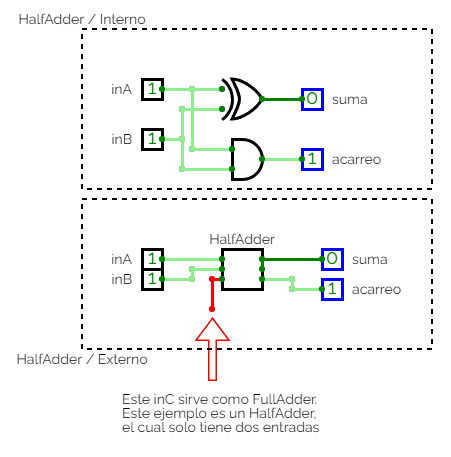
\includegraphics[width=0.75\linewidth]{ALU/HalfAdder.png}
            \caption{Esquema interior/exterior del circuito HalfAdder}
            \label{fig:h_adder}
        \end{figure}
    \subsection{Implementación HDL}
        \begin{figure}[H]
            \centering
            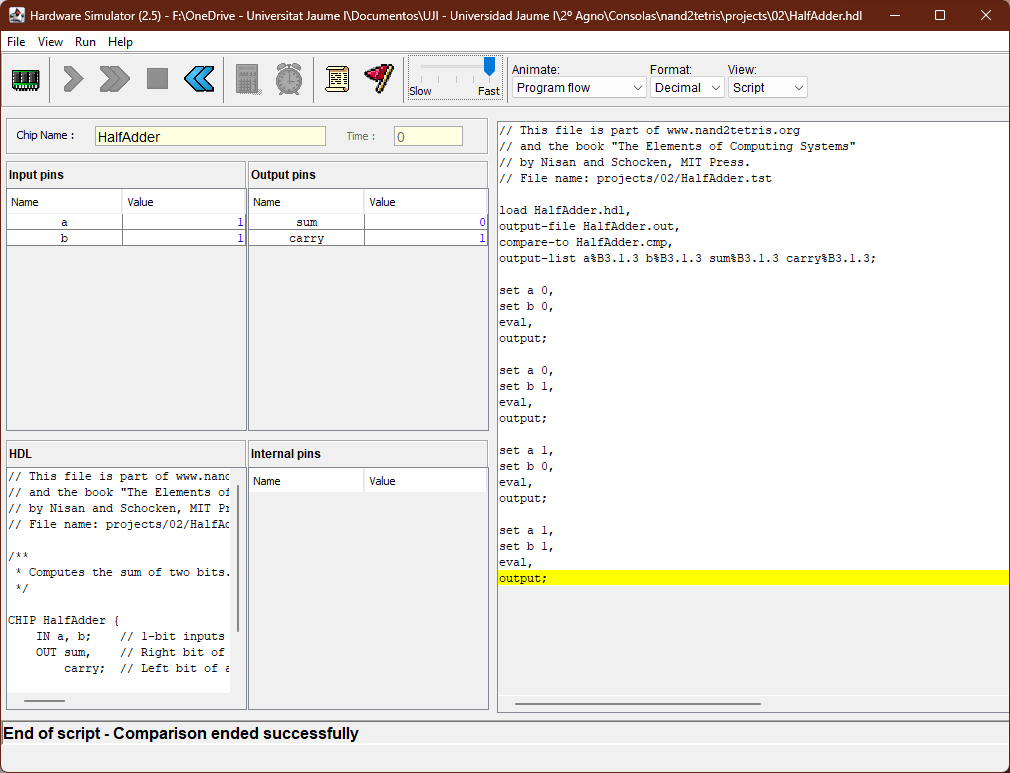
\includegraphics[width=0.75\linewidth]{ALU/halfadder_hw.png}
            \caption{Test de HalfAdder}
            \label{fig:enter-label}
        \end{figure}
        \subsubsection{Archivo .HDL}
            \begin{lstlisting}
        CHIP HalfAdder {
        IN a, b;    // 1-bit inputs
        OUT sum,    // Right bit of a + b 
            carry;  // Left bit of a + b
    
        PARTS:
            Xor(a=a,b=b,out=sum);
            And(a=a,b=b,out=carry);
        }
            \end{lstlisting}
            \newpage
        \subsubsection{Archivo .TST}
    \begin{lstlisting}
    load HalfAdder.hdl,
    output-file HalfAdder.out,
    compare-to HalfAdder.cmp,
    output-list a%B3.1.3 b%B3.1.3 sum%B3.1.3 carry%B3.1.3;
    
    set a 0,
    set b 0,
    eval,
    output;
    
    set a 0,
    set b 1,
    eval,
    output;
    
    set a 1,
    set b 0,
    eval,
    output;
    
    set a 1,
    set b 1,
    eval,
    output;

    \end{lstlisting}
        \subsubsection{Archivo .CMP}
    \begin{lstlisting}
    |   a   |   b   |  sum  | carry |
    |   0   |   0   |   0   |   0   |
    |   0   |   1   |   1   |   0   |
    |   1   |   0   |   1   |   0   |
    |   1   |   1   |   0   |   1   |
    \end{lstlisting}
\newpage
%%%%%%%%%%%%%%%%%%%%%%%%%%%%%%%%%%%%%%%%%%%%%%%%%%%%%%%%%%%%%%%%%%%%%%%%%%
%%%%%%%%%%%%%%%%%%%%%%%%%%%%%%%%%%%%%%%%%%%%%%%%%%%%%%%%%%%%%%%%%%%%%%%%%%
\section{FullAdder}
    \subsection{Tabla de verdad y explicación del circuito}
        EL FullAdder actúa como un Half exceptuando que contiene 3 inputs (3 bits). Su circuito se compone de 2 HalfAdders y se selecciona si contiene acarreo con una puerta OR. 
        \begin{table}[H]
            \centering
            \caption{Tabla de verdad de Full Adder}
            \label{tab:fulladder}
            \begin{tblr}{
              width = \linewidth,
              colspec = {Q[77]Q[77]Q[133]Q[279]Q[287]},
              hline{1,10} = {-}{0.08em},
              hline{2,7} = {-}{},
            }
            A & B & Cin & Sum (S) & Cout (C) \\
            0 & 0 & 0   & 0       & 0        \\
            0 & 0 & 1   & 1       & 0        \\
            0 & 1 & 0   & 1       & 0        \\
            0 & 1 & 1   & 0       & 1        \\
            1 & 0 & 0   & 1       & 0        \\
            1 & 0 & 1   & 0       & 1        \\
            1 & 1 & 0   & 0       & 1        \\
            1 & 1 & 1   & 1       & 1        
            \end{tblr}
        \end{table}

    \subsection{Esquema del circuito exterior y exterior} 
        \begin{figure}[H]
            \centering
            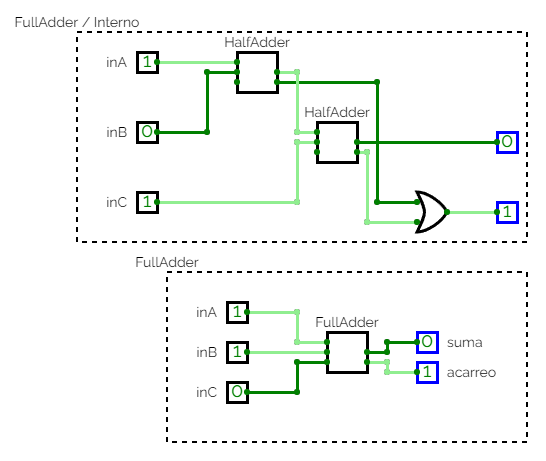
\includegraphics[width=0.75\linewidth]{ALU/FullAdder.png}
            \caption{Esquema interior/exterior del circuito FullAdder}
            \label{fig:f_adder}
        \end{figure}
    \subsection{Implementación HDL}
        \begin{figure}[H]
            \centering
            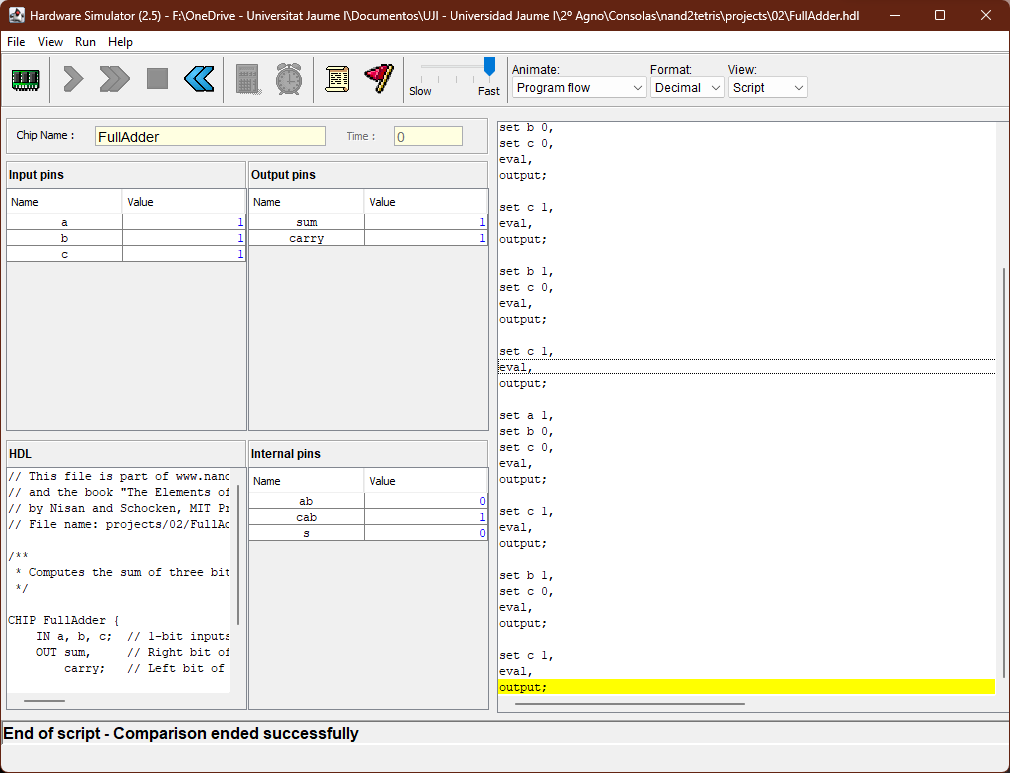
\includegraphics[width=0.75\linewidth]{ALU/fulladder_hw.png}
            \caption{Test de FullAdder}
            \label{fig:enter-label}
        \end{figure}
        \subsubsection{Archivo .HDL}
            \begin{lstlisting}
        CHIP FullAdder {
            IN a, b, c;  // 1-bit inputs
            OUT sum,     // Right bit of a + b + c
                carry;   // Left bit of a + b + c
        
            PARTS:
                HalfAdder(a=a,b=b,sum=ab,carry=cab);
                HalfAdder(a=c,b=ab,sum=sum,carry=s);
                Or(a=cab,b=s,out=carry);
        }
            \end{lstlisting}
        \subsubsection{Archivo .TST}
            \begin{lstlisting}
        load FullAdder.hdl,
        output-file FullAdder.out,
        compare-to FullAdder.cmp,
        output-list a%B3.1.3 b%B3.1.3 c%B3.1.3 sum%B3.1.3 carry%B3.1.3;
        
        set a 0,
        set b 0,
        set c 0,
        eval,
        output;
        
        set c 1,
        eval,
        output;
        
        set b 1,
        set c 0,
        eval,
        output;
        
        set c 1,
        eval,
        output;
        
        set a 1,
        set b 0,
        set c 0,
        eval,
        output;
        
        set c 1,
        eval,
        output;
        
        set b 1,
        set c 0,
        eval,
        output;
        
        set c 1,
        eval,
        output;

            \end{lstlisting}
        \subsubsection{Archivo .CMP}
            \begin{lstlisting}
        |   a   |   b   |   c   |  sum  | carry |
        |   0   |   0   |   0   |   0   |   0   |
        |   0   |   0   |   1   |   1   |   0   |
        |   0   |   1   |   0   |   1   |   0   |
        |   0   |   1   |   1   |   0   |   1   |
        |   1   |   0   |   0   |   1   |   0   |
        |   1   |   0   |   1   |   0   |   1   |
        |   1   |   1   |   0   |   0   |   1   |
        |   1   |   1   |   1   |   1   |   1   |
            \end{lstlisting}
\newpage
%%%%%%%%%%%%%%%%%%%%%%%%%%%%%%%%%%%%%%%%%%%%%%%%%%%%%%%%%%%%%%%%%%%%%%%%%%
%%%%%%%%%%%%%%%%%%%%%%%%%%%%%%%%%%%%%%%%%%%%%%%%%%%%%%%%%%%%%%%%%%%%%%%%%%
\section{Add16}
    \subsection{Tabla de verdad y explicación del circuito}
        El Add16 actúa como un adder, cuyo propósito es hacer la operación de suma con dos inputs de 16 bits. Funciona conectando varios FullAdders. 
        % \usepackage{color}
        % \usepackage{tabularray}
        \begin{table}[H]
        \centering
        \caption{Tabla de verdad de Add16}
        \label{tab:fulladder}
        \begin{tblr}{
          width = \linewidth,
          colspec = {Q[133]Q[135]Q[135]Q[196]Q[96]Q[217]},
          cells = {c, font=\ttfamily}, % Set font to monospaced (typewriter)
          vlines,
          hline{1,10} = {-}{0.08em},
          hline{2} = {-}{},
        }
        Inputs  & $A$ & $B$ & $C_{in}$ & Sum & $C_{out}$ \\
        Input 1 & 0   & 0   & 0      & 0   & 0       \\
        Input 2 & 0   & 0   & 1      & 1   & 0       \\
        Input 3 & 0   & 1   & 0      & 1   & 0       \\
        Input 4 & 0   & 1   & 1      & 0   & 1       \\
        Input 5 & 1   & 0   & 0      & 1   & 0       \\
        Input 6 & 1   & 0   & 1      & 0   & 1       \\
        Input 7 & 1   & 1   & 0      & 0   & 1       \\
        Input 8 & 1   & 1   & 1      & 1   & 1       
        \end{tblr}
        \end{table}
    \subsection{Esquema del circuito exterior y exterior}
        \subsubsection{Exterior}
            \begin{figure}[H]
                \centering
                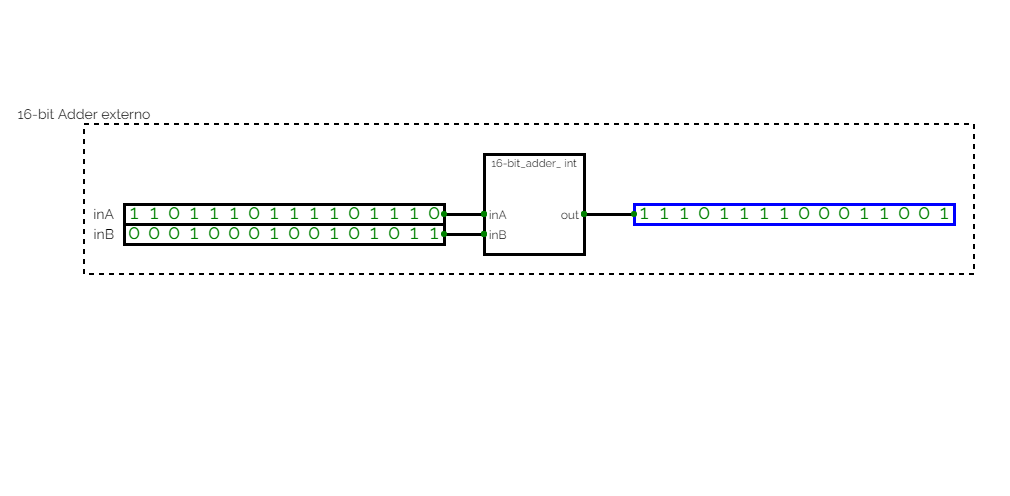
\includegraphics[width=0.75\linewidth]{ALU/16-bit_adder_ext.png}
                \caption{Esquema exterior del circuito Add16}
                \label{fig:add16}
            \end{figure}
        \subsubsection{Interior} 
        \begin{figure}[H]
            \centering
            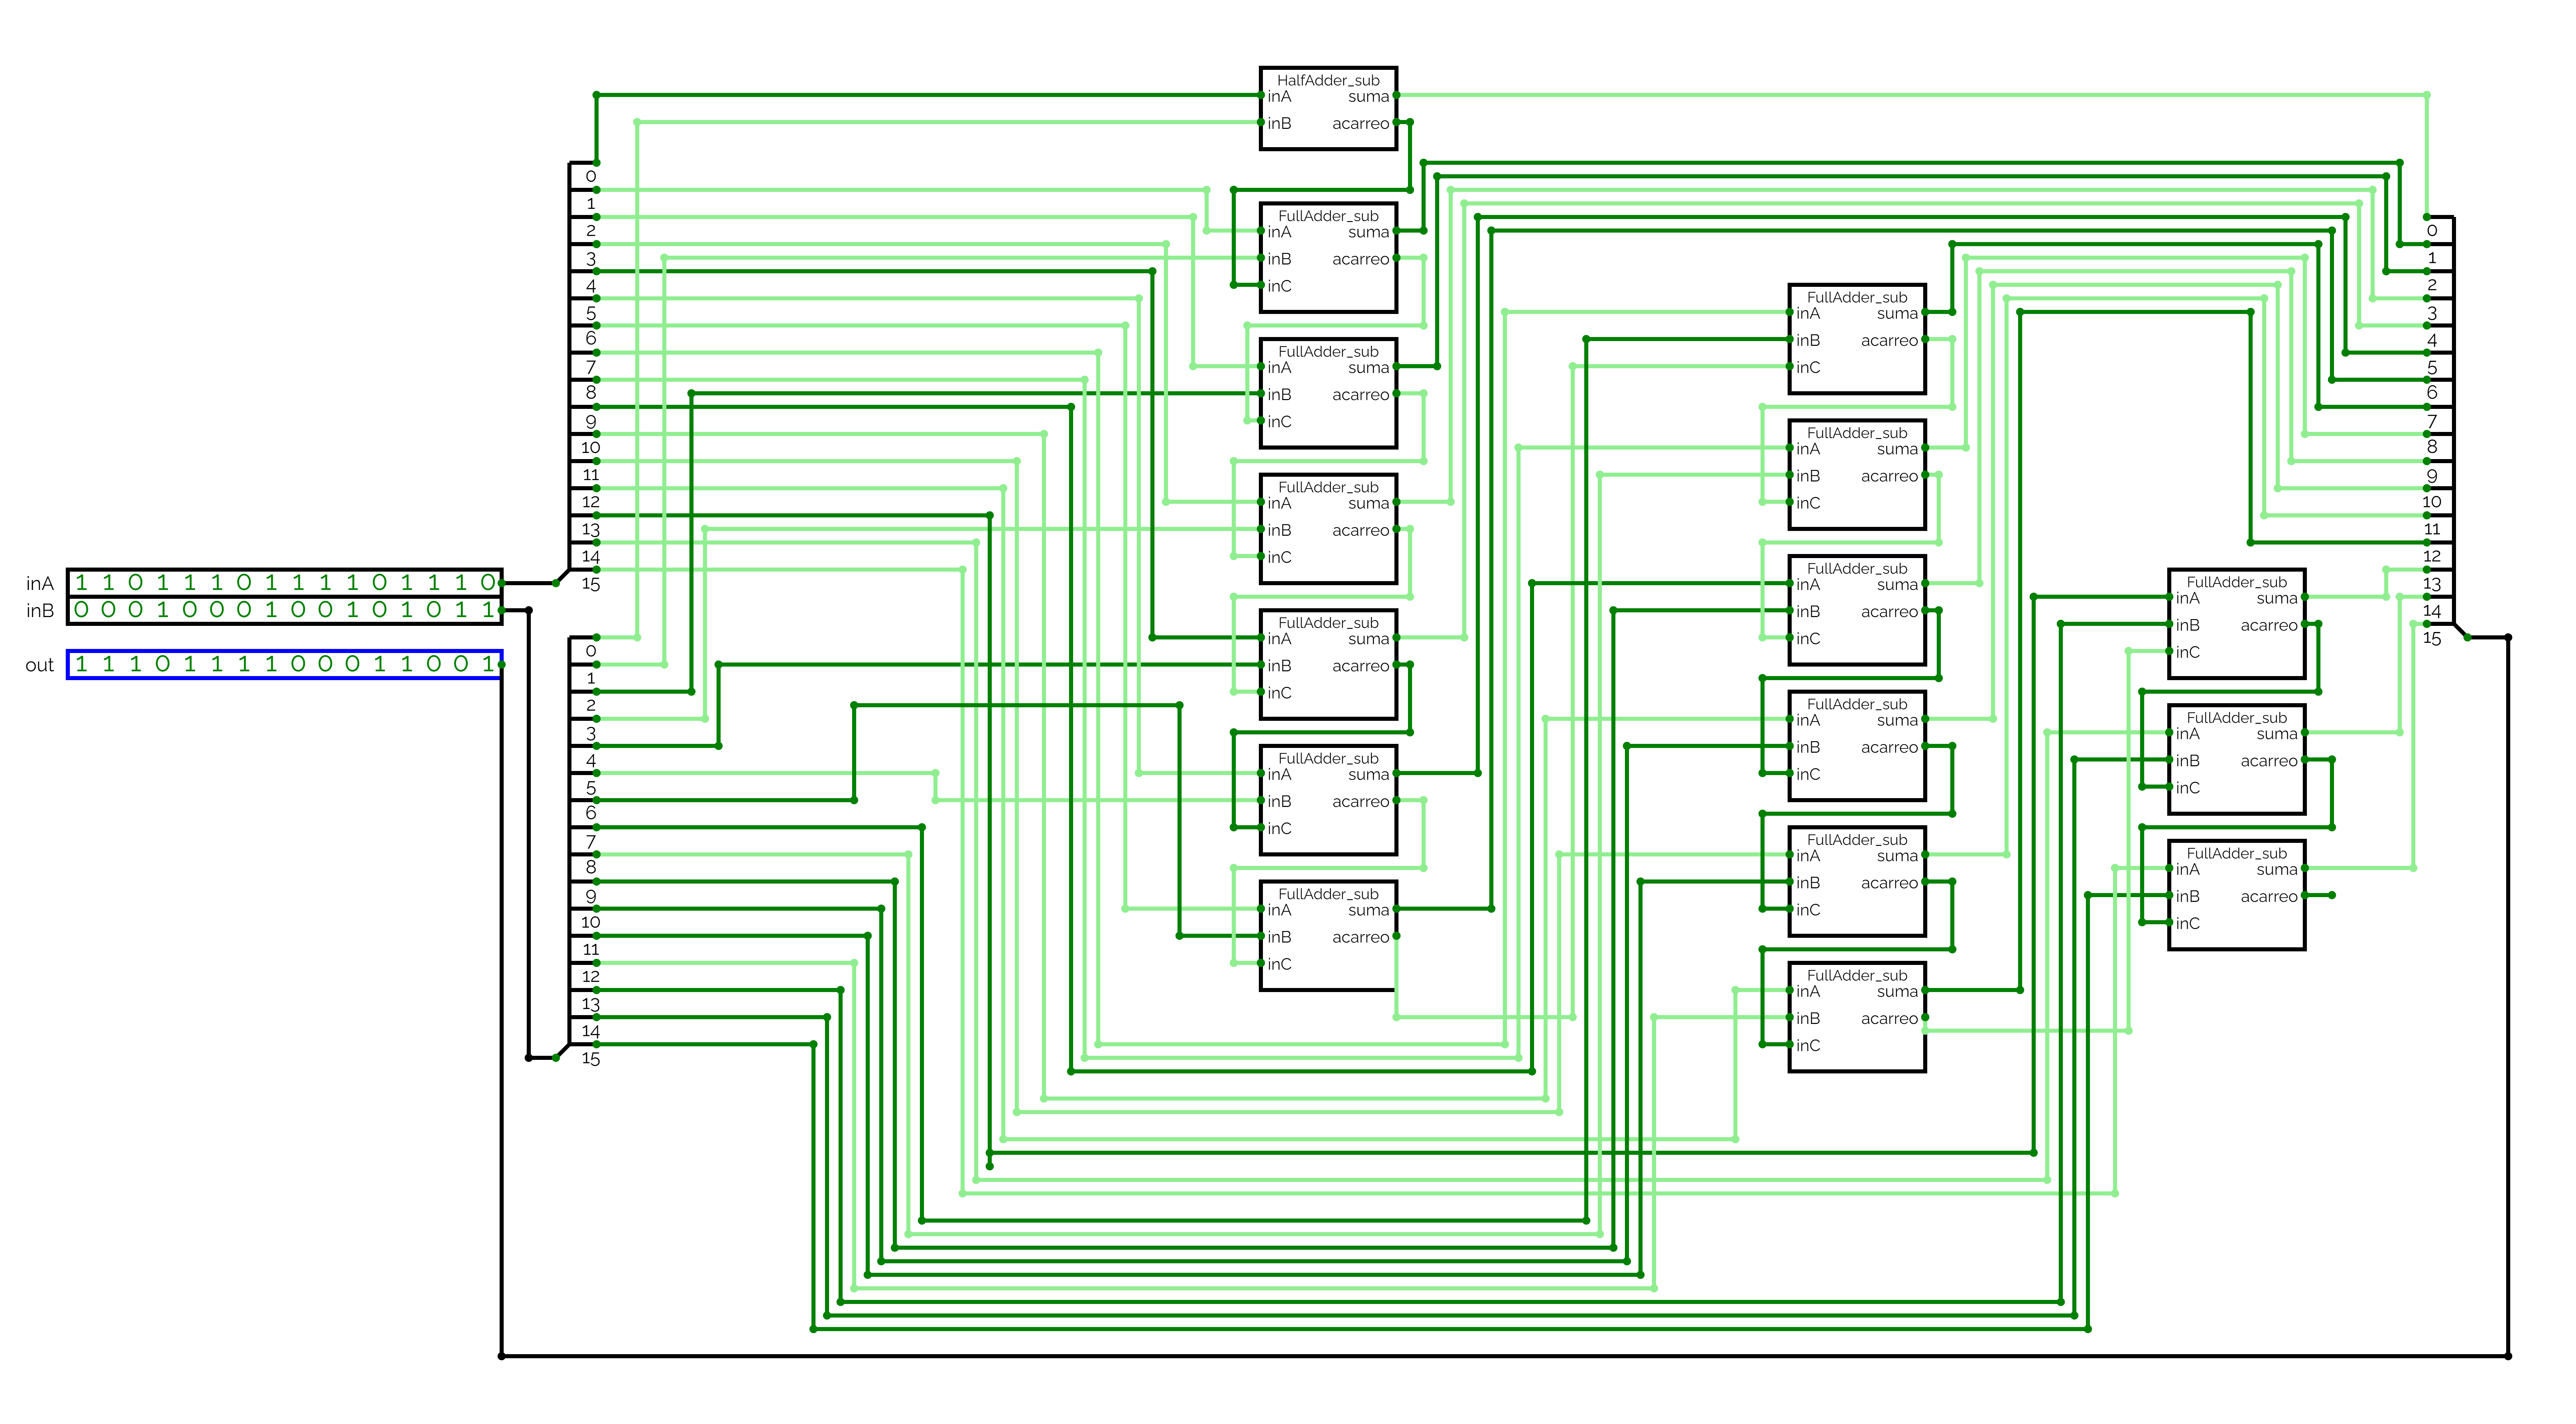
\includegraphics[width=0.75\linewidth]{ALU/16-bitadder_ int.png}
            \caption{Esquema interior del circuito Add16}
            \label{fig:f_add16}
        \end{figure}
    \subsection{Implementación HDL}
    \begin{figure}[H]
        \centering
        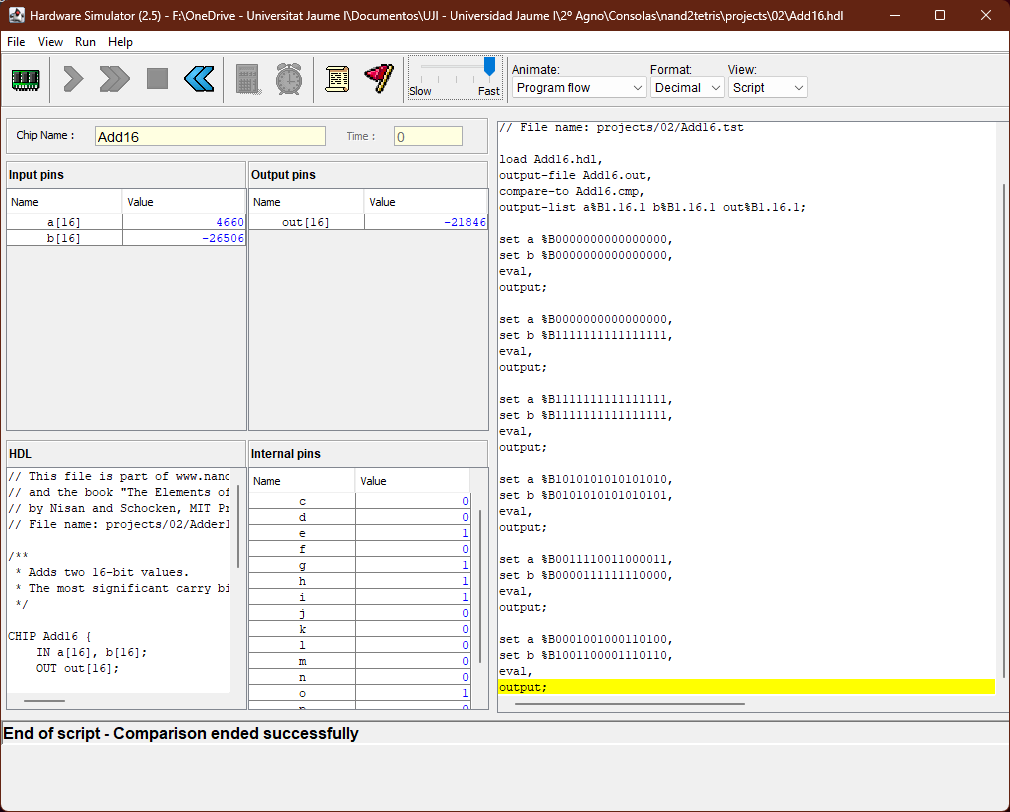
\includegraphics[width=0.75\linewidth]{ALU/add16_hw.png}
        \caption{Test de Add16}
        \label{fig:enter-label}
    \end{figure}
    \newpage
        \subsubsection{Archivo .HDL}
            \begin{lstlisting}
                
        CHIP Add16 {
            IN a[16], b[16];
            OUT out[16];
        
            PARTS:	
                HalfAdder(a=a[0],b=b[0],sum=out[0],carry=c);
                FullAdder(a=a[1],b=b[1],c=c,sum=out[1],carry=d);
                FullAdder(a=a[2],b=b[2],c=d,sum=out[2],carry=e);
                FullAdder(a=a[3],b=b[3],c=e,sum=out[3],carry=f);
                FullAdder(a=a[4],b=b[4],c=f,sum=out[4],carry=g);
                FullAdder(a=a[5],b=b[5],c=g,sum=out[5],carry=h);
                FullAdder(a=a[6],b=b[6],c=h,sum=out[6],carry=i);
                FullAdder(a=a[7],b=b[7],c=i,sum=out[7],carry=j);
                FullAdder(a=a[8],b=b[8],c=j,sum=out[8],carry=k);
                FullAdder(a=a[9],b=b[9],c=k,sum=out[9],carry=l);
                FullAdder(a=a[10],b=b[10],c=l,sum=out[10],carry=m);
                FullAdder(a=a[11],b=b[11],c=m,sum=out[11],carry=n);
                FullAdder(a=a[12],b=b[12],c=n,sum=out[12],carry=o);
                FullAdder(a=a[13],b=b[13],c=o,sum=out[13],carry=p);
                FullAdder(a=a[14],b=b[14],c=p,sum=out[14],carry=q);
                FullAdder(a=a[15],b=b[15],c=q,sum=out[15],carry=drop);
        }
            \end{lstlisting}
        \subsubsection{Archivo .TST}
        \begin{lstlisting}
            
        set a %B0000000000000000,
        set b %B0000000000000000,
        eval,
        output;
        
        set a %B0000000000000000,
        set b %B1111111111111111,
        eval,
        output;
        
        set a %B1111111111111111,
        set b %B1111111111111111,
        eval,
        output;
        
        set a %B1010101010101010,
        set b %B0101010101010101,
        eval,
        output;
        
        set a %B0011110011000011,
        set b %B0000111111110000,
        eval,
        output;
        
        set a %B0001001000110100,
        set b %B1001100001110110,
        eval,
        output;

        \end{lstlisting}
    

        \subsubsection{Archivo .CMP}
        \begin{lstlisting}
            
    |        a         |        b         |       out        |
    | 0000000000000000 | 0000000000000000 | 0000000000000000 |
    | 0000000000000000 | 1111111111111111 | 1111111111111111 |
    | 1111111111111111 | 1111111111111111 | 1111111111111110 |
    | 1010101010101010 | 0101010101010101 | 1111111111111111 |
    | 0011110011000011 | 0000111111110000 | 0100110010110011 |
    | 0001001000110100 | 1001100001110110 | 1010101010101010 |
        \end{lstlisting}
\newpage
%%%%%%%%%%%%%%%%%%%%%%%%%%%%%%%%%%%%%%%%%%%%%%%%%%%%%%%%%%%%%%%%%%%%%%%%%%
%%%%%%%%%%%%%%%%%%%%%%%%%%%%%%%%%%%%%%%%%%%%%%%%%%%%%%%%%%%%%%%%%%%%%%%%%%
\section{Inc16}
    \subsection{Tabla de verdad y explicación del circuito}
        El incrementer es, en pocas palabras, un adder con dos inputs; uno con un número binario de 16-bits y otro con el valor constante de 1. Así que, funciona incrementando el valor A por 1. 
        \begin{table}[H]
        \centering
        \caption{Tabla de verdad de Inc16}
        \label{tab:fulladder}
        \begin{tblr}{
          width = \linewidth,
          colspec = {Q[471]Q[469]},
          cells = {c, font=\ttfamily}, % Set font to monospaced (typewriter)
          hlines,
          vlines,
          hline{1,6} = {-}{0.08em},
        }
        \texttt{Inputs (A15-A0)}                  & \texttt{Outputs (B15-B0)}                 \\
        \texttt{0000 0000 0000 0000 (Decimal: 0)} & \texttt{0000 0000 0000 0001 (Decimal: 1)} \\
        \ldots                                   & \ldots                                    \\
        \texttt{1111 1111 1111 1110 (Decimal: 65534)} & \texttt{1111 1111 1111 1111 (Decimal: 65535)} \\
        \texttt{1111 1111 1111 1111 (Decimal: 65535)} & \texttt{0000 0000 0000 0000 (Decimal: 0)}   
        \end{tblr}
        \end{table}

    \subsection{Esquema del circuito exterior y exterior}
        
        \subsubsection{Interior} 
        \begin{figure}[H]
            \centering
            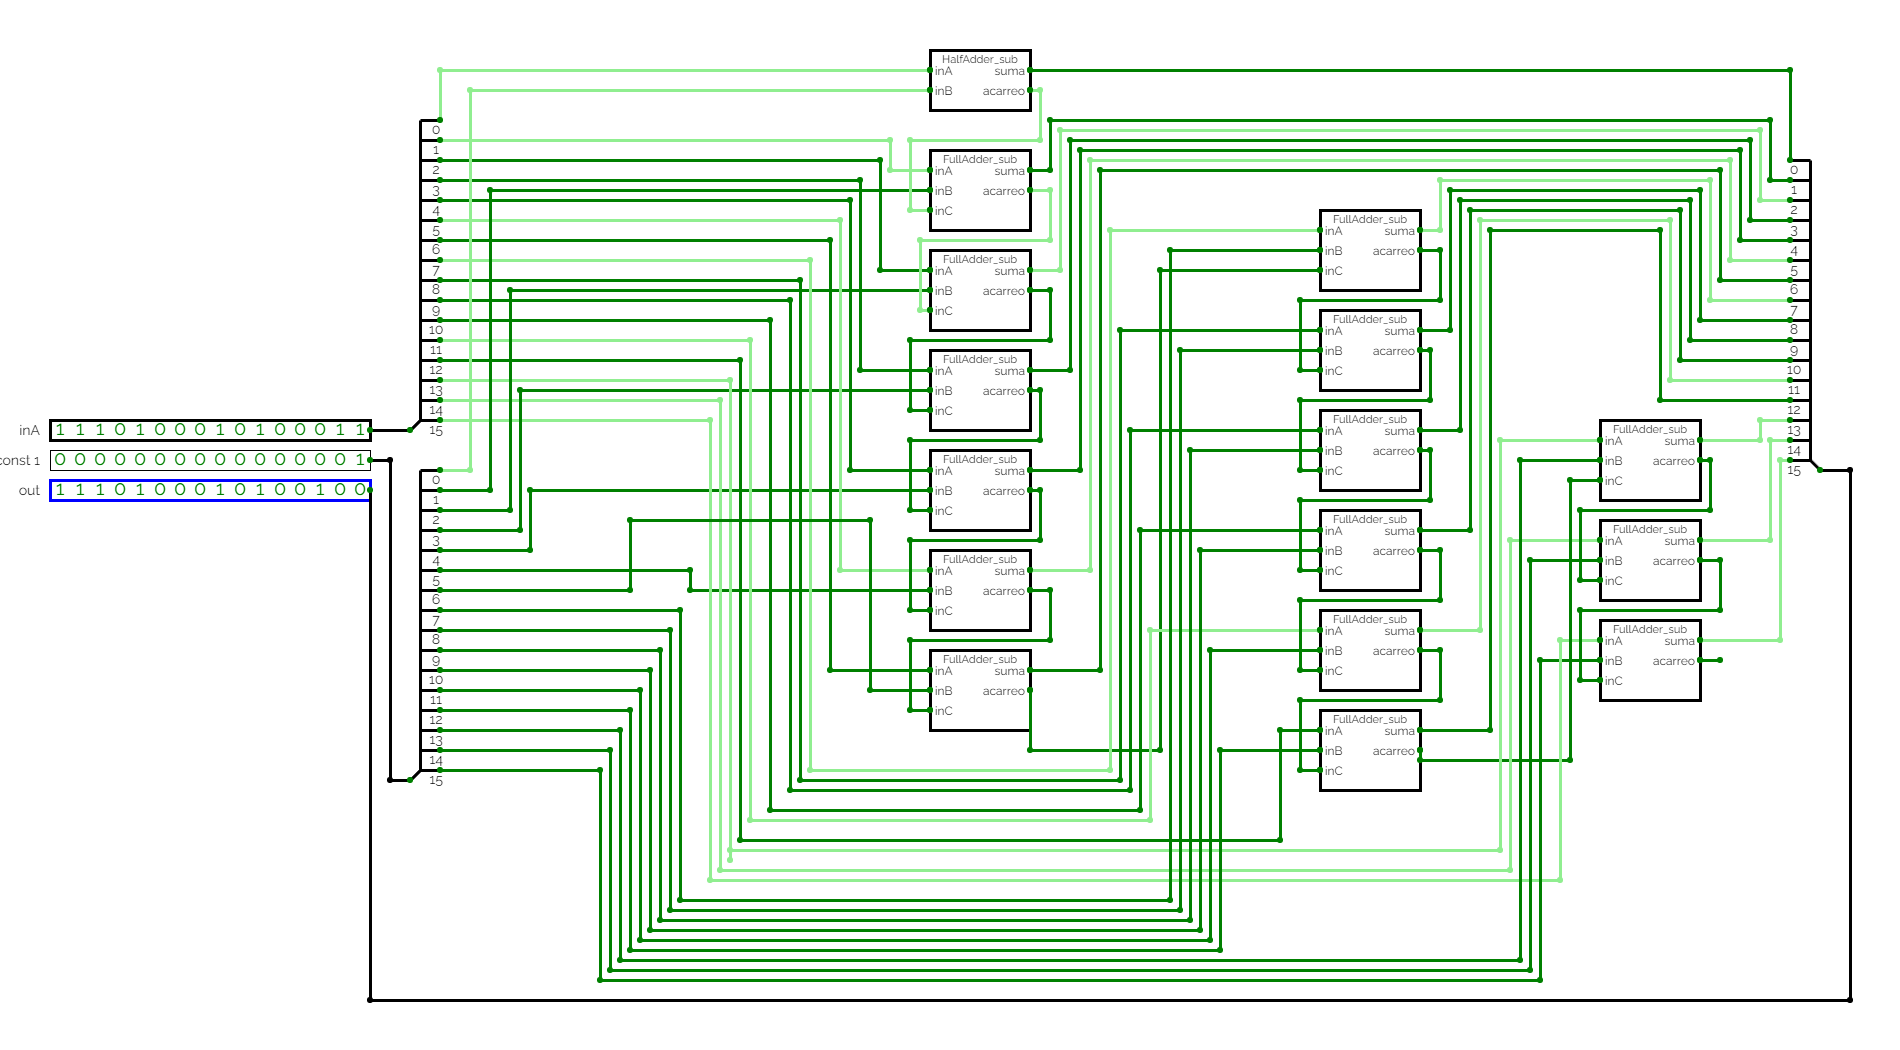
\includegraphics[width=0.75\linewidth]{ALU/Incrementer_int.png}
            \caption{Esquema interior del circuito Inc16}
            \label{fig:f_Inc16}
        \end{figure}
    \subsection{Implementación HDL}
    \begin{figure}[H]
        \centering
        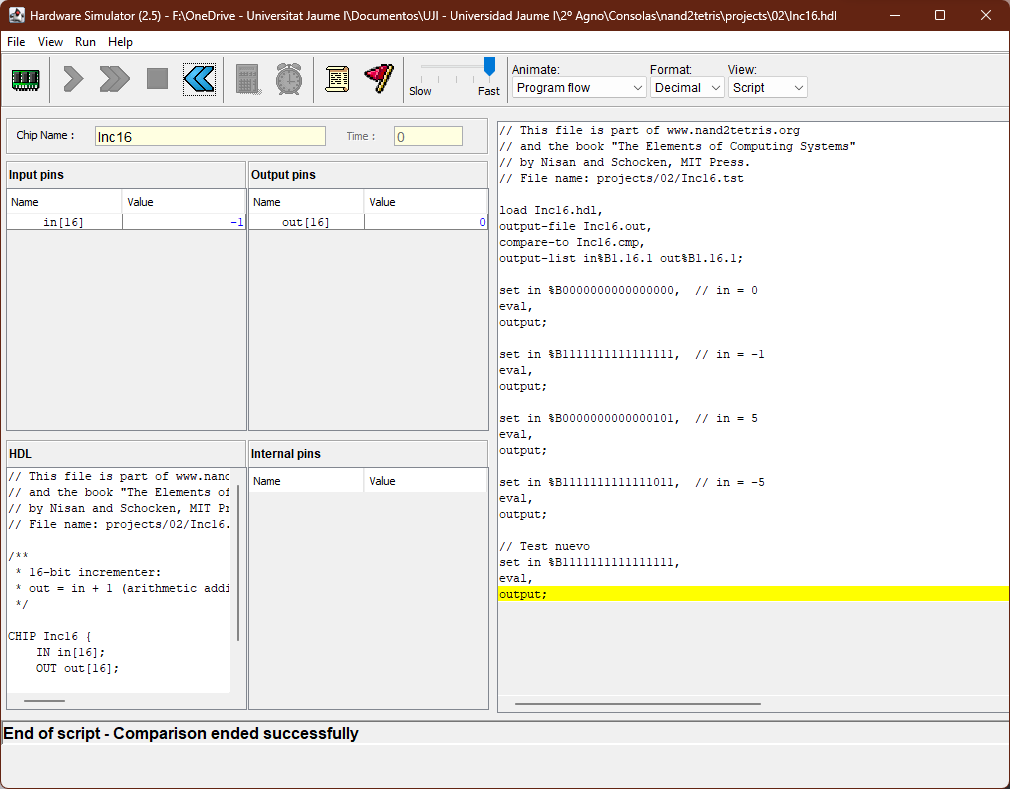
\includegraphics[width=0.75\linewidth]{ALU/inc16_hw.png}
        \caption{Test de Inc16}
        \label{fig:enter-label}
    \end{figure}
        \subsubsection{Archivo .HDL}
            \begin{lstlisting}
                
        CHIP Inc16 {
            IN in[16];
            OUT out[16];
        
            PARTS:
            Add16(a=in,b[0]=true,out=out);
        }
            \end{lstlisting}
        \subsubsection{Archivo .TST}
        \begin{lstlisting}

        load Inc16.hdl,
        output-file Inc16.out,
        compare-to Inc16.cmp,
        output-list in%B1.16.1 out%B1.16.1;
        
        set in %B0000000000000000,  // in = 0
        eval,
        output;
        
        set in %B1111111111111111,  // in = -1
        eval,
        output;
        
        set in %B0000000000000101,  // in = 5
        eval,
        output;
        
        set in %B1111111111111011,  // in = -5
        eval,
        output;
        
        // Test nuevo
        set in %B1111111111111111,
        eval,
        output;


        \end{lstlisting}

        \subsubsection{Archivo .CMP}
        \begin{lstlisting}
        |        in        |       out        |
        | 0000000000000000 | 0000000000000001 |
        | 1111111111111111 | 0000000000000000 |
        | 0000000000000101 | 0000000000000110 |
        | 1111111111111011 | 1111111111111100 |
        | 1111111111111111 | 0000000000000000 |
        \end{lstlisting}
\newpage
%%%%%%%%%%%%%%%%%%%%%%%%%%%%%%%%%%%%%%%%%%%%%%%%%%%%%%%%%%%%%%%%%%%%%%%%%%
%%%%%%%%%%%%%%%%%%%%%%%%%%%%%%%%%%%%%%%%%%%%%%%%%%%%%%%%%%%%%%%%%%%%%%%%%%
\section{ALU}
    \subsection{Tabla de verdad y explicación del circuito}
        La ALU lleva a cabo diferentes operaciones dependiendo del bit que lleven sus multiples inputs. 
        % \usepackage{color}
        % \usepackage{tabularray}
        \begin{table}[H]
        \centering
        \caption{Tabla de verdad de Add16}
        \label{tab:fulladder}
        \begin{tblr}{
          width = \linewidth,
          colspec = {Q[123]Q[67]Q[94]Q[96]Q[185]Q[285]Q[83]},
          cells = {c, font=\ttfamily}, % Set font to monospaced (typewriter)
          cell{1}{1} = {c=2}{0.19\linewidth},
          cell{1}{3} = {c=2}{0.19\linewidth},
          hline{1,13} = {-}{0.08em},
          hline{2,4} = {-}{},          
        }
        {Estos bits dicen \\como preajustar \\el input x} &  & {Estos bits dicen\\como preajustar\\el input x } &  & {El bit seleciona~\\entre + / And} & {Este bit selecciona como\\producir el output} & \\
        zx & nx & zy & ny & f & no & out\\
        {if zx then\\x = 0} & {if nx\\then\\x=!x} & {if zy\\then\\y=0} & {if ny\\then\\y=!y} & {if f then\\out=x+y\\else\\out=xy} & {if no\\then\\out=!out} & f(x,y)=\\
        0 & 1 & 1 & 1 & 1 & 1 & x+1\\
        1 & 1 & 0 & 1 & 1 & 1 & y+1\\
        0 & 0 & 1 & 1 & 1 & 0 & x-1\\
        1 & 1 & 0 & 0 & 1 & 0 & y-1\\
        0 & 0 & 0 & 0 & 1 & 0 & x+y\\
        0 & 1 & 0 & 0 & 1 & 1 & x-y\\
        0 & 0 & 0 & 1 & 1 & 1 & y-x\\
        0 & 0 & 0 & 0 & 0 & 0 & xy\\
        0 & 1 & 0 & 1 & 0 & 1 & x\textbar{}y
        \end{tblr}
        \end{table}
    \subsection{Esquema del circuito exterior y exterior} 
            \subsubsection{Exterior}
            \begin{figure}[H]
                \centering
                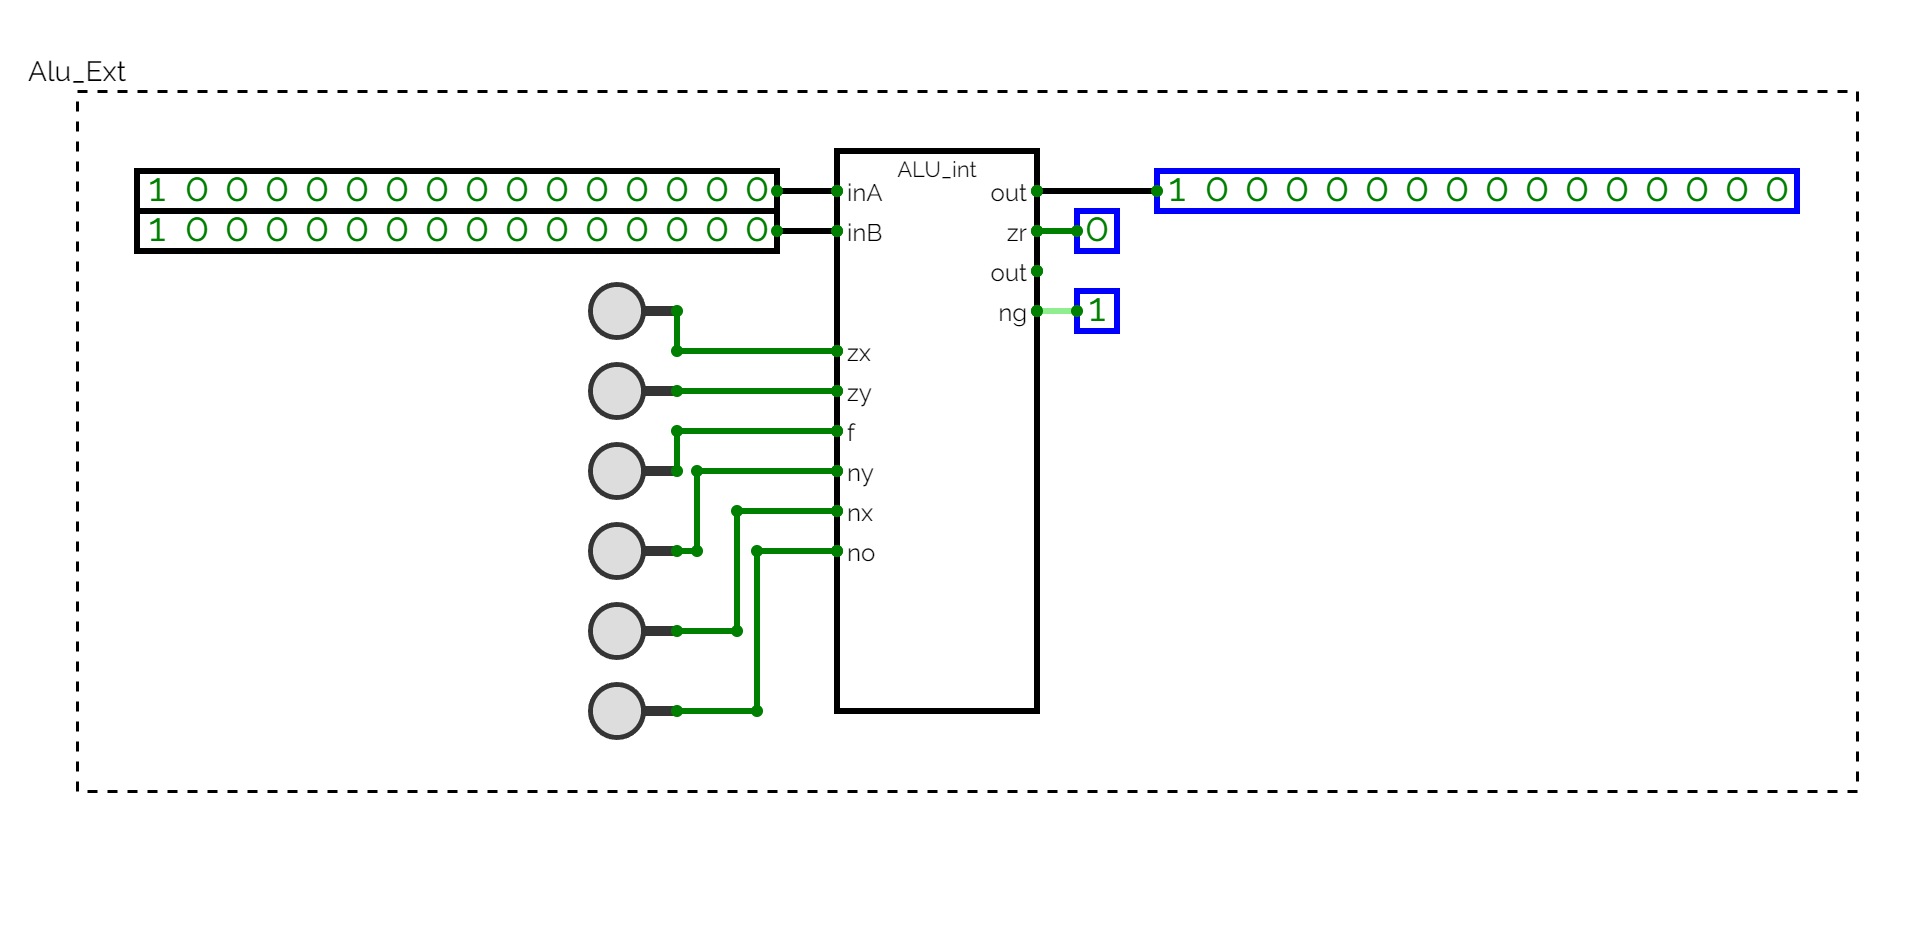
\includegraphics[width=0.75\linewidth]{ALU/ALU_ext.png}
                \caption{Esquema exterior de una ALU}
                \label{fig:Inc16}
            \end{figure}
        \subsubsection{Interior} 
        \begin{figure}[H]
            \centering
            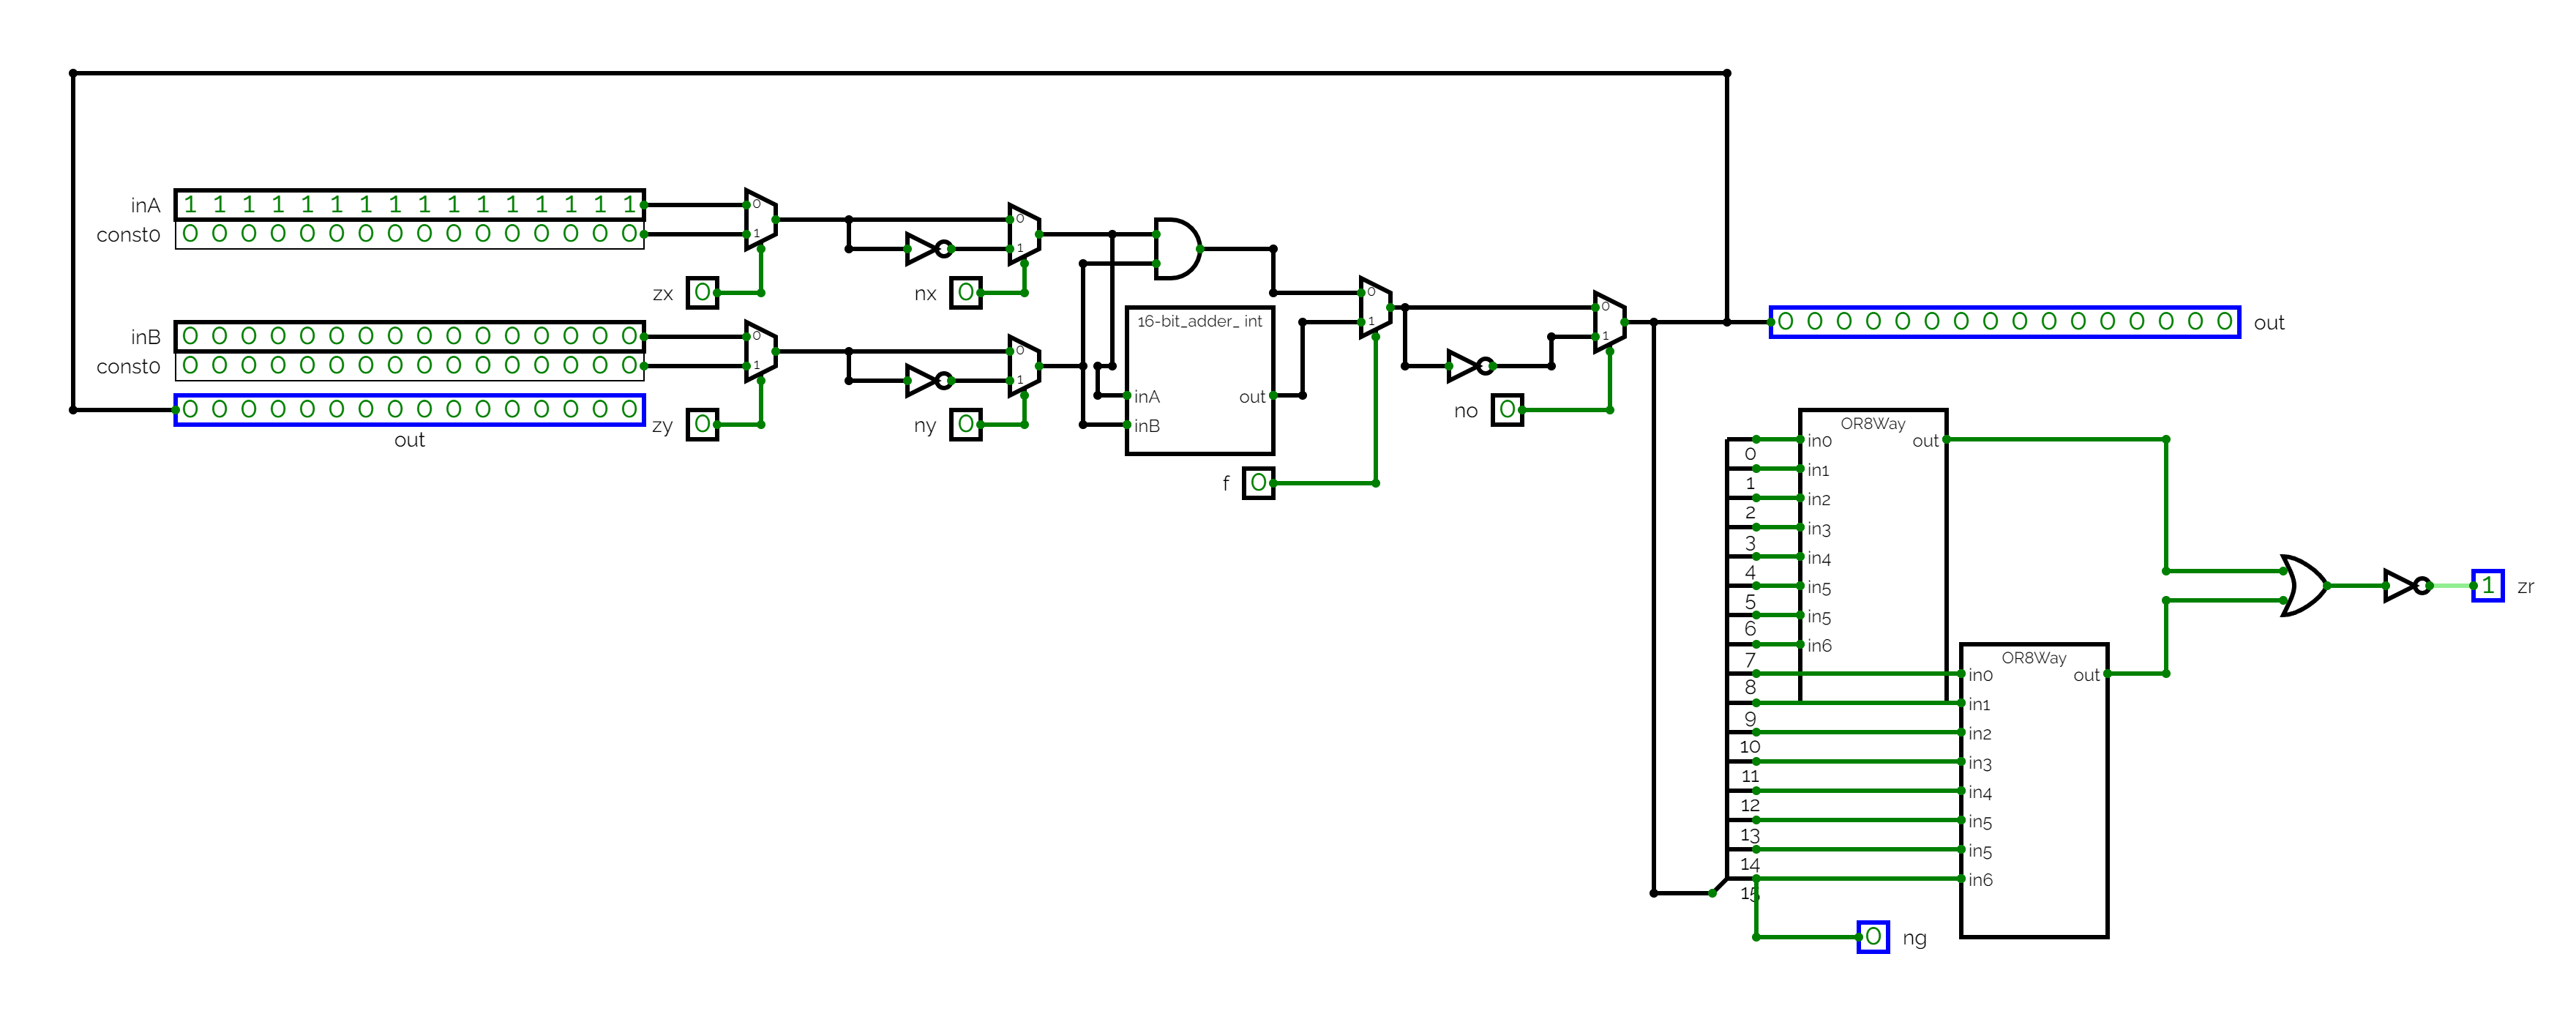
\includegraphics[width=0.75\linewidth]{ALU/ALU_int.png}
            \caption{Esquema interior de una ALU}
            \label{fig:f_Inc16}
        \end{figure}
    \subsection{Implementación HDL}
    \begin{figure}[H]
        \centering
        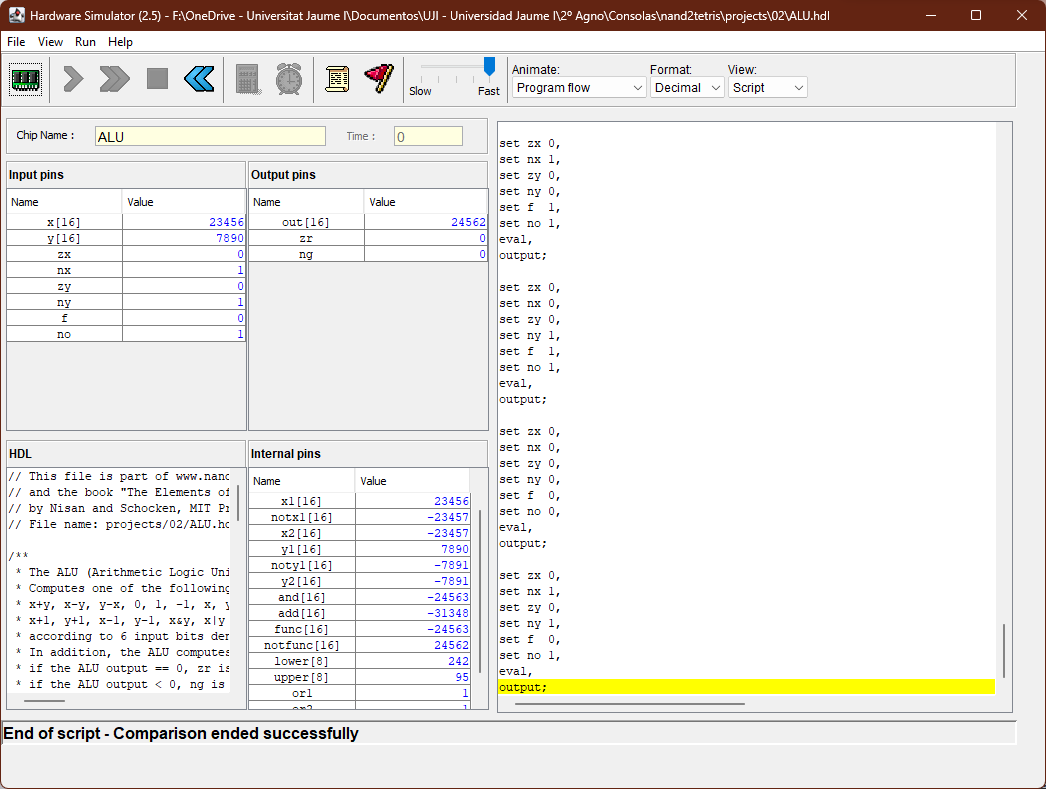
\includegraphics[width=0.75\linewidth]{ALU/alu_hw.png}
        \caption{Test de ALU}
        \label{fig:enter-label}
    \end{figure}
        \subsubsection{Archivo .HDL}
            \begin{lstlisting}
        CHIP ALU {
            IN
                x[16], y[16],  // 16-bit inputs
                zx, // zero the x input?
                nx, // negate the x input?
                zy, // zero the y input?
                ny, // negate the y input?
                f,  // compute  out = x + y (if f == 1) or out = x & y (if == 0)
                no; // negate the out output?
        
            OUT
                out[16], // 16-bit output
                zr, // 1 if (out == 0), 0 otherwise
                ng; // 1 if (out < 0),  0 otherwise
        
            PARTS:
            // zx
            Mux16(a=x, b=false, sel=zx, out=x1);
        
            // nx
            Not16(in=x1, out=notx1);
            Mux16(a=x1, b=notx1, sel=nx, out=x2);
        
            // zy
            Mux16(a=y, b=false, sel=zy, out=y1);
        
            // ny
            Not16(in=y1, out=noty1);
            Mux16(a=y1, b=noty1, sel=ny, out=y2);
        
            // f
            And16(a=x2, b=y2, out=and);
            Add16(a=x2, b=y2, out=add);
            Mux16(a=and, b=add, sel=f, out=func);
        
            // no, ng
            Not16(in=func, out=notfunc);
            Mux16(a=func, b=notfunc, sel=no, out=out, out[0..7]=lower, out[8..15]=upper, out[15]=ng);
        
            // zr
            Or8Way(in=lower, out=or1);
            Or8Way(in=upper, out=or2);
            Or(a=or1, b=or2, out=or);
            Not(in=or, out=zr);
        }
            \end{lstlisting}
        \subsubsection{Archivo .TST}
\begin{lstlisting}
    // Tests viejos
    . . .
    // Test nuevo
    set x %B0000000000000000,  // x = 0
    set y %B1111111111111111,  // y = -1
    
    // Operacion AND
    set zx 1,
    set nx 0,
    set zy 1,
    set ny 0,
    set f  0,
    set no 0,
    eval,
    output;}
\end{lstlisting}    
        \subsubsection{Archivo .CMP}
\begin{lstlisting}
    // Comparers viejos
    ...
    // Comprarer nuevo
    |        x         |        y         |zx |nx |zy |ny | f |no |       out        |zr |ng |
    | 0000000000000000 | 1111111111111111 | 1 | 0 | 1 | 0 | 0 | 0 | 0000000000000000 | 1 | 0 |
\end{lstlisting}
\newpage
%%%%%%%%%%%%%%%%%%%%%%%%%%%%%%%%%%%%%%%%%%%%%%%%%%%%%%%%%%%%%%%%%%%%%%%%%%
%%%%%%%%%%%%%%%%%%%%%%%%%%%%%%%%%%%%%%%%%%%%%%%%%%%%%%%%%%%%%%%%%%%%%%%%%%

\printbibliography[heading=bibintoc]
\end{document}
